\documentclass[letterpaper, 10pt]{report}
\title{Clemson Hack Pack}
\author{Clemson ACM}
\date{\today}

\usepackage{makeidx}
\usepackage{multicol}
\usepackage{geometry}
\usepackage{tabularx}
\usepackage{pdfpages}
\geometry{margin=1in}

% Pad out huge chapter numbers in the TOC
\usepackage{tocloft}

% Custom command for inline code.
\newcommand{\code}[1]{\texttt{#1}}

% Paragraph spacing should be easy!
\usepackage{parskip}

% Chapter title format: "X. Chaptertitle", not "Chapter X\nChaptertitle".
% Also, make \sections stand out a bit more.
\usepackage{titlesec}
\titleformat{\chapter}[block]{\normalfont\huge\bfseries}{\thechapter.}{1em}{\Huge}
\titleformat{\section}[block]{\normalfont\large\bfseries}{\thesection.}{1em}{\LARGE}

% Adjust spacing around headers to reduce empty space
\titlespacing*{\chapter}{0pt}{-22pt}{-1pt}
\titlespacing*{\section}{0pt}{10pt}{0pt}
\titlespacing*{\subsection}{0pt}{10pt}{0pt}
\titlespacing*{\subsubsection}{0pt}{0pt}{0pt}

% Citations should use superscript. It's nice.
\usepackage[superscript, biblabel]{cite}

% Use the Bera font family (based on Bitstream Vera) for text (bera), captions
% (berasans), and code (beramono).
\usepackage{bera}
\usepackage[scaled]{berasans}
\usepackage[scaled]{beramono}
\usepackage[T1]{fontenc}

% Needed for the inclusion of graphics.
\usepackage{graphicx}

% Allows the use of EPS files, a type of vector graphic.
\usepackage{epstopdf}

% Use the listings package for pretty source code inclusions.
\usepackage{color}
\usepackage{xcolor}
\usepackage{soul}
\usepackage{listings}
\lstset{
  basicstyle=\footnotesize\ttfamily, % Use a truetype, footnote-sized font.
  numbers=left,                      % line numbers go on the left
  numbersep=10pt,                    % how far the line-numbers are from the code
  tabsize=2,                         % sets default tabsize to 2 spaces
  extendedchars=true,                % lets you use non-ASCII characters; for 8-bits encodings only
  breaklines=true,                   % sets automatic line breaking
  keywordstyle=\bfseries,            % Keyword styling
  numberstyle=\ttfamily\color{gray}, % the style that is used for the line-numbers
  stringstyle=\color{gray},          % string literal style
  commentstyle=\itshape\color{gray}, % comment literal style
  title=\lstname,                    % show the filename of files included with \lstinputlisting
  frame=b,                           % show a frame along the bottom
  rulecolor=\color{lightgray},
  language=C++,                      % the default language of the code
  showspaces=false,                  % show spaces as space, not a litle underscore.
  showstringspaces=false             % same as above, in strings.
  showtabs=false,                    % same as above, with tabs.
  xleftmargin=17pt,
  framexleftmargin=17pt,
  framexrightmargin=5pt
}

% Listings caption configuration.
\usepackage{caption}
\DeclareCaptionFont{white}{\color{white}}
\DeclareCaptionFormat{listing}{\colorbox[cmyk]{0.43, 0.35, 0.35,0.01}{\parbox{\textwidth}{\vspace{1.5pt}\hspace{10pt}#1#2#3}}}
\captionsetup[lstlisting]{format=listing,labelfont=white,textfont=white, singlelinecheck=false, margin=0pt, font={bf, sf}}

% Defines a tikz frame for page-broken listing hints.
% Shamelessly stolen from https://tex.stackexchange.com/questions/77996/how-to-show-a-hint-when-lstlisting-is-breaking-page
\usepackage[framemethod=tikz]{./formatting/mdframed}
\mdfdefinestyle{note}
  {
    hidealllines = true ,
    skipabove    = .5\baselineskip ,
    skipbelow    = .5\baselineskip ,
    singleextra  = {} ,
    firstextra   = {
      \node[right,overlay,align=center,font=\continuingfont]
        at (O) {\continuingtext};
    } ,
    secondextra  = {
      \node[above right,overlay,align=left,font=\continuingfont]
        at (O |- P) {\continuedtext};
    } ,
    middleextra  = {
      \node[right,overlay,align=left,font=\continuingfont]
        at (O) {\continuingtext};
      \node[above right,overlay,align=left,font=\continuingfont]
        at (O |- P) {\continuedtext};
    }
  }

% Sets up the hint content and style for page-broken listings.
\newcommand*\continuingfont{\color{gray}\footnotesize\itshape}
\newcommand*\continuingtext{Continues on next page}
\newcommand*\continuedtext{Continued from previous page}

% A wrapper command for automatically wrapping input listings
% with a hintable frame.
\newcommand{\acmlisting}[2][]
{
\mdframed[style=note]
\lstinputlisting[#1]{#2}
\endmdframed
}

% Turn on the powerful indexing features
\makeindex

% Make links, footnotes, etc. clickable, and generate pdf bookmarks.
\usepackage{hyperref}
\hypersetup{
  pdfauthor={Clemson ACM, acm@cs.clemson.edu},
  pdfcreator={Clemson ACM, acm@cs.clemson.edu},
  pdftitle={Clemson ACM Hack Pack},
  pdfsubject={Clemson ACM Hack Pack},
  unicode=true,
  colorlinks=false,
  pdfborder=0 0 0,
  bookmarks=true
}



\begin{document}
\maketitle

\begingroup
\let\clearpage\relax
\chapter*{10 Commandments of ACM Contests}
\begin{center}Paraphrased from Dr. Dean\end{center}
\begin{multicols}{2}
\begin{enumerate}
    \item Thou shalt sort first and ask questions later
    \item Thou shalt know the STL and use it well
    \item Thou shalt know thy algorithms by heart
    \item Thou shalt brute force $\leq$ 10 million items
    \item Thou shalt when in doubt solve with DP
    \item Thou shalt never count by 1
    \item Thou shalt reinitialize thy data structures
    \item Thou shalt test often and submit early
    \item Thou shalt never trust a sample input
    \item Thou shalt print according to the output spec
\end{enumerate}
\end{multicols}
\begin{center}
Remember what the Dr. said\\
"Algorithms are Cool!"
\end{center}

\endgroup


\tableofcontents

\chapter{Basic Data Structures}
\section{Set}\index{Set!Ordered Set}
Sets are data structures that are useful for determining if an element has been seen before or not.
Sets are ordered\index{Ordered} collections of elements typically implemented as a balanced binary search tree.
They have unique keys\index{Unique Keyed}; that is to say that there are no duplicates in a set.
However, unlike an array, elements are referenced by their ordering\index{Associative}, not their position in the data structure.

%Will use LaTeX cross referencing tools as soon as these sections are written.
#ifdef hackpackpp
See `unordered\_set' for a version of the set that does not have an order, but is based on hash tables.
See `multiset' for a version of the set that is not uniquely keyed.
See `unordered\_multiset' for a version of the set that does not have an order and is also not uniquely keyed.
#endif

\subsection{Reference}
\acmlisting[caption=Set Reference, label=Set Reference]{./structures/set/set.cpp}

#ifdef hackpackpp
\subsection{Applications}

\begin{itemize}
	\item Determining how many and what items are in one set and also in another (intersection).
	\item Determining how many and what items are in one set but \emph{not} in another (difference).
	\item Determining how many and what items are in either sets (union).
	\item Filtering out non-unique inputs.
    %Will cross reference when possible
    \item Can be useful for sweep line approaches
\end{itemize}
#endif

#ifdef hackpackpp
\subsection{Example Contest Problem: Cow Pens}
Farmer John's cows keep wandering off into the hills to learn cowculus from nomadic mathematicians.
Unappreciative of refined bovine arithmetic, Farmer John decides to fence in his cows to keep them from escaping.

He wants to build the fence without crossing over any of the trees on his property (which the cows claim are valuable for studying graph theory), and he'd like the fence to be rectangular (a perfect shape, the cows say).
One side of the rectangle should be formed by the river at the southern edge of Farmer John's property, so that the cows can contemplate wave-based trigonometric functions (and stay hydrated).

Please compute the maximum area that Farmer John can enclose with a fence that meets the above requirements.
You can assume that the river has the position $Y=0$ and Farmer John's property lies north of the river.

\subsubsection{Input Format}
\begin{itemize}
	\item Line 1: One integer, $N$, $(N < 1000000)$, specifying the number of trees in the field.
	\item Lines 2..$(N+1)$: Each line contains two integers $X$ and $Y$ $(0 <= X,Y <= 1000000)$.
		Each pair corresponds to the location of one tree in Farmer John's field.
\end{itemize}

\subsubsection{Sample Input}
\acmlisting[caption=Cow Pens Input, label=Cow Pens Input]{./structures/set/problems/cowpens/cowpens.in}

\subsubsection{Output Format}
\begin{itemize}
  \item Line 1: One integer that represents the area of the largest possible rectangle that Farmer John can build.
\end{itemize}

\subsubsection{Sample Output}
\acmlisting[caption=Cow Pens Output, label=Cow Pens Output]{./structures/set/problems/cowpens/cowpens.out}
\subsubsection{Example Solution}
#endif

#ifdef hackpack
\subsection{In Sweeplines}
#endif
\acmlisting[caption=Cow Pens Solution, label=Cow Pens Solution]{./structures/set/problems/cowpens/cowpens.cpp}

#ifdef hackpackpp
\subsubsection{Lessons Learned}
\begin{itemize}
	\item The STL Set can be used as a basic binary search tree.
	\item Write comparison functions to change orderings of Sets, Maps, and the \code{sort()} function.
	\item \code{typedef} long type names to something shorter for ease of use.
	\item Sometimes it is better to \emph{modify} the input than to code edge cases.
	\item \code{lower\_bound} returns an iterator pointing to the first element $\leq$ the searched element.
\end{itemize}
#endif

#ifdef hackpackpp
\subsection{Example Contest Problem: The Cows Form a Union}
The cows have formed a union, and have gone on strike to protest Farmer John's new cow pen.

Each cow has been given a unique union ID number, painted on its side.
The three cows with the smallest, closest ID numbers just so happen to be the union bosses.

Farmer John, in an effort to track union activity, took two photographs of cow rallies that he's sure the bosses attended, but he's not sure which cows are the bosses.
Using the ID numbers of all the cows in the photographs, please determine the three cows that have the closest ID numbers so that Farmer John can attempt to negotiate with them.
In case several sets of cows have equally close ID numbers, choose the set that contains the lowest ID number.
You can assume that there are at least three cows between the two pictures.

\subsubsection{Input Format}
\begin{itemize}
	\item Line 1: A space-delimited list, ending with $0$, of $N$ ID numbers $(0 \leq N \leq 1000000)$. 
		Each number $i_n$ $(0 < i_{0..N-1} \leq 1000000)$ indicates that a cow with that ID number is present in the \emph{first} photograph.
	\item Line 2: A space-delimited list, ending with $0$, of $N$ ID numbers $(0 \leq N \leq 1000000)$. 
		Each number $i_n$ $(0 < i_{0..N-1} \leq 1000000)$ indicates that a cow with that ID number is present in the \emph{second} photograph.
\end{itemize}

\subsubsection{Sample Input}
\acmlisting[caption=The Cows Form a Union Input, label=The Cows Form a Union Input]{./structures/set/problems/union/union.in}

\subsubsection{Output Format}
\begin{itemize}
	\item Line 1: Three space-delimited integers in ascending order, indicating the three cows who lead the union.
\end{itemize}

\subsubsection{Sample Output}
\acmlisting[caption=The Cows Form a Union Output, label=The Cows Form a Union Output]{./structures/set/problems/union/union.out}
\subsubsection{Example Solution}
#endif

#ifdef hackpack
\subsection{Finding a Union}
#endif
\acmlisting[caption=The Cows Form a Union Solution, label=The Cows Form a Union Solution]{./structures/set/problems/union/union.cpp}

#ifdef hackpackpp
\subsection{Example Contest Problem: Cow Distances}
As a result of the cows' lobbying efforts, the federal government is investigating Farmer John for possible violations of the Magnanimous Agricultural Defense of Cloven Ochlophobic Workers Statute, which states that any two cows of differing breeds (Farmer John owns Guernseys and Holsteins) must be given an inter-breed comfort zone of at least 1.000 meters.
Cows of the same breed are allowed to mingle as cozily as they wish.

Assuming the regulators know the precise location of every cow in Farmer John's field, please help the federal government determine whether or not to crack down on Farmer John's gross oppression of his herd.

\subsubsection{Input Format}
\begin{itemize}
	\item Line 1: One integer $G$, $(G < 500000)$, specifying the number of Guernseys to follow.
	\item Line 2..$(G+1)$: Two integers $X$ and $Y$, $0 \leq X,Y \leq 1000000$.
		Each pair corresponds to the location of one Guernsey in the field.
	\item Line $(G+2)$: One integer, $H$, $(H < 500000)$, specifying the number of Holsteins to follow. 
	\item Line $(G+3)$..$(G+H+2)$: Two integers $X$ and $Y$, $0 \leq X,Y \leq 1000000$.
		Each pair corresponds to the location of one Holstein in the field.
\end{itemize}

\subsubsection{Sample Input}
\acmlisting[caption=Cow Distances Input, label=Cow Distances Input]{./structures/set/problems/closest/closest.in}

\subsubsection{Output Format}
\begin{itemize}
	\item Line 1: the number $1$ if Farmer John is breaking the law or $0$ if he is not.
\end{itemize}

\subsubsection{Sample Output}
\acmlisting[caption=Cow Distances Output, label=Cow Distances Output]{./structures/set/problems/closest/closest.out}
#endif


\section{Map}
Maps are Associative, Ordered, Mapped, Uniquely Keyed, and Allocator aware\cite{cplusplus}.
Mapped means that each key corresponds to a specific value. Use it to record relationships in data.
\acmlisting[caption=Map Reference, label=Map Reference]{./structures/map/map.cpp}

\section{Heap}\index{heap}\index{priority\_queue}
Heaps are very useful data structures that support at least the following operations:

\begin{itemize}
	\item Insert.
	\item Remove the smallest element.
\end{itemize}

Many other implementations also implement a decrease key operation and delete operation.

The standard library provides a two sets of functions that provide this functionality.
The first is the \lstinline{priority_queue} data structure found in the queue header.
The second is the \lstinline{make_heap} functions in found the algorithm header.
Neither of these implementations strictly implements the decrease key operation.
The code sample shown below shows how to create a binary min heap as well as the heap sort algorithm which runs in $O(N \log N)$ time.

\subsection{Reference}
\acmlisting[caption=Heap Reference, label=Heap Reference]{./structures/heap/heap.cpp}

\subsection{Applications}
\begin{itemize}
	\item Dijkstra's Algorithm
	\item Prim's Algorithm
	\item Priority Based Queuing
\end{itemize}

\section{Graph}
Graphs are useful for a variety of different real world problems.
Graphs are comprised of Nodes and Edges.
Nodes represent a distinct state.
Edges represent the possible transitions between states.
Graphs can be directed(edges are one way) or undirected(edges are the same going to or from a node).

Paths are graphs that have no branches off.
Cycles are graphs that connect back on them selves.
Trees are graphs that contain no cycles.
Forests are graphs that contain multiple disjoint trees.
Bipartite Graphs have a set of "source" nodes and a set of "edge" nodes

Two nodes $i,j$ are said to be connected if there is a path from i to j.
Two nodes $i,j$ are said to be strongly connected if there is a directed path from i to j and j to i.

\subsection{Reference}
\acmlisting[caption= Undirected Graph, label=Undirected Graph]{./structures/graph/graph.cpp}

\subsection{Applications}
For all run times, $V$ is the number of nodes, and $E$ is the number of edges.
\begin{itemize}
	\item Shortest Paths
		\begin{itemize}
			\item Breath First Search --- Graphs with equal weight edges $O(V+E)$
			\item Dijkstra's Algorithm --- Graphs with non-negative edges weights $O(E \log V)$.
			\item Bellman Ford --- Graphs with some negative edges $O(VE)$
			\item Floyd Warshall --- Graphs with negative edges but not cycles $O(V^3)$.
			\item Dynamic Programming --- Directed Acyclic Graphs various running times.
		\end{itemize}
	\item Minimum Spanning Trees 
		\begin{itemize}
			\item Prim's Algorithm --- For undirected graphs; if run for each component, finds the minimum spanning forest$O(E \log V)$.
			\item Kruskal's Algorithm --- For graphs; finds the minimum spanning forests in unconnected graphs $(E \log V)$
		\end{itemize}
	\item Similarity/Connectivity
		\begin{itemize}
			\item Depth First Search --- Find (Strongly) Connected Components $O(V+E)$
			\item Depth First Search --- Find a path from i to j $O(V+E)$
		\end{itemize}
	\item Topological Sorting 
		\begin{itemize}
			\item Depth First Search --- Use start and stop times to topologically sort $O(V+E)$
		\end{itemize}
	\item Matchings
		\begin{itemize}
			\item Greedy --- Many of these problems can be solved by a greedy max/min flow algorithm in $O(EV \log V \log F)$ where F is is the max flow.
		\end{itemize}
	\item Flow/Routing
		\begin{itemize}
			\item Greedy --- Many of these problems can be solved by a greedy max/min flow algorithm in $O(EV \log V \log F)$ where F is is the max flow.
		\end{itemize}
	\item Clustering
	\item Centrality
\end{itemize}

#ifdef hackpackpp
\subsection{Sample Contest Problem, The Cows Escape}
Farmer John's Farm has become infested with Zombies!
Farmer John being slightly out of shape wants to take the shortest amount of time to escape the zombies.

Farmer John's Farm is laid out in squares.
Being prepared, Farmer John has his Early Zombie Detection System that will alert him to the rating of the zombies in these squares.
Based off his research into the topic, Farmer John knows based on the rating how long it will take to evade the zombies in that sector.

Help Farmer John find the shortest time it will take Farmer John to escape his farm with his cows.

\subsubsection{Input Format}
\begin{itemize}
	\item Line 1:One integer $T$ indicating the number of test cases to evaluate
	\item Line 2:Three integers $k,w,h$ representing the number zombie classes to follow and the width and height of Farmer John's Farm
	\item Lines 3..$(3+k)$: The letter representing the zombie class, it will not be `F' and the time it will take to evade them, $t$
	\item Lines $(4+k)$..$(4+k+h)$: $W$ capital letters representing the zombie classes in each sector of farmer John's farm.  Farmer John's initial position is designated by `F'.
\end{itemize}

\subsubsection{Sample Input}
\acmlisting[caption=The Cows Escape Sample Input, label= The Cows Escape Sample Input]{./structures/graph/problems/escape/escape.in}

\subsubsection{Output Format}
\begin{itemize}
	\item Line 1:  1 integer per line for each test case representing the minimum time it takes to escape the farm.
\end{itemize}

\subsubsection{Sample Output}
\acmlisting[caption=The Cows Escape Sample Output, label= The Cows Escape Sample Output]{./structures/graph/problems/escape/escape.out}
\subsubsection{Sample Solution}
#endif

#ifdef hackpack
\subsection{Dijkstra in a graph}
#endif
\acmlisting[caption=The Cows Escape Sample Solution, label= The Cows Escape Sample Solution]{./structures/graph/problems/escape/escape.cpp}

#ifdef hackpackpp
\subsubsection{Lessons Learned}
\begin{itemize}
	\item Dijkstra can be solved using a priority queue using $O(N \log N)$ time.
\end{itemize}
#endif



\chapter{Algorithms}
\section{Dijkstra's Algorithm}\index{Shortest Path!Dijkstra}
Dijkstra's Algorithm solves the single-source shortest path problem of finding the shortest paths between the source 
node and all other nodes in a connected graph with non-negative edge path costs.  
The graph can be both directed and undirected.  
It is commonly used to find the shortest path between a source and destination node.  
For graphs with negative weights, see Bellman-Ford Algorithm.
It is commonly inplemented using a priority queue and runs in $O(E \log V)$.

\subsection{Applications}

\begin{itemize}
	\item  Finding the shortest paths between a source node and all other nodes in a connected graph with non-negative edge path costs.
\end{itemize}

\subsection{Example Contest Problem: Farm Tour\cite{farmtour}}
When Farmer John's friends visit him on the farm, he likes to show them around. 
His farm comprises $N$ $(1 \leq N \leq 1000)$ fields numbered $1..N$, the first of which contains his house and the Nth of which contains the big barn. 
A total $M$ $(1 \leq M \leq 10000)$ paths that connect the fields in various ways. 
Each path connects two different fields and has a nonzero length smaller than $35,000$. 

To show off his farm in the best way, he walks a tour that starts at his house, potentially travels through some fields, and ends at the barn. 
Later, he returns (potentially through some fields) back to his house again. 

He wants his tour to be as short as possible, however he doesn't want to walk on any given path more than once. 
Calculate the shortest tour possible. 
Farmer John is sure that some tour exists for any given farm.

\subsubsection{Input Format}
\begin{itemize}
	\item Line $1$: Two space-separated integers: $N$ and $M$. 
	\item Lines $2..M+1$: Three space-separated integers that define a path: The starting field, the end field, and the path's length. 
\end{itemize}

\subsubsection{Sample Input}
\acmlisting[caption=Farm Tour Input, label=Farm Tour Input]{./algorithms/dijkstra/problems/farm-tour/farmtour.in}

\subsubsection{Output Format}
\begin{itemize}
	\item Line 1: A single line containing the length of the shortest tour. 
\end{itemize}

\subsubsection{Sample Output}
\acmlisting[caption=Farm Tour Output, label= Farm Tour Output]{./algorithms/dijkstra/problems/farm-tour/farmtour.out}

\subsection{Example Contest Problem: Milk Routing\cite{milkroute}}
Farmer John's farm has an outdated network of $M$ pipes $(1 \leq M \leq 500)$ for pumping milk from the barn to his milk storage tank.  
He wants to remove and update most of these over the next year, but he wants to leave exactly one path worth of pipes intact, 
so that he can still pump milk from the barn to the storage tank.

The pipe network is described by N junction points $(1 \leq N \leq 500)$, each of which can serve as the endpoint of a set of pipes.  
Junction point 1 is the barn, and junction point N is the storage tank.  
Each of the M bi-directional pipes runs between a pair of junction points, and has an associated latency 
(the amount of time it takes milk to reach one end of the pipe from the other) and capacity (the amount of milk per unit time
that can be pumped through the pipe in steady state).  
Multiple pipes can connect between the same pair of junction points.

For a path of pipes connecting from the barn to the tank, the latency of the path is the sum of the latencies of the pipes along 
the path, and the capacity of the path is the minimum of the capacities of the pipes along the path (since this is the "bottleneck" 
constraining the overall rate at which milk can be pumped through the path).  
If Farmer John wants to send a total of $X$ units of milk through a path of pipes with latency $L$ and capacity $C$, the time this takes is therefore $L + X/C$.

Given the structure of Farmer John's pipe network, please help him select a single path from the barn to the storage tank that will allow him to pump $X$ units
of milk in a minimum amount of total time.

Official Solution: \url{http://www.usaco.org/current/current/data/sol_mroute.html}

\subsubsection{Input Format}
\begin{itemize}
	\item Line $1$: Three space-seperated integers: $N$ $M$ $X$ $(1 \leq X \leq 1,000,000)$.
	\item Line $2..1+M$: Each line describes a pipe using 4 integers: $I$ $J$ $L$ $C$.
			$I$ and $J$ $(1 \leq I,J \leq N)$ are the juntion points at both ends of the pipe.
			$L$ and $C$ $(1 \leq L,C \leq 1,000,000)$ give the latency and capacity of the pipe.
\end{itemize}

\subsubsection{Sample Input}
\acmlisting[caption=Milk Routing Input, label=Milk Routing Input]{./algorithms/dijkstra/problems/milk-routing/milkrouting.in}

\subsubsection{Output Format}
\begin{itemize}
	\item Line 1: The minimum amount of time it will take Farmer John to send milk along a single path, 
			rounded down to the nearest integer.
\end{itemize}

\subsubsection{Sample Output}
\acmlisting[caption=Milk Routing Output, label=Milk Routing Output]{./algorithms/dijkstra/problems/milk-routing/milkrouting.out}

\subsection{Example Contest Problem: Dueling GPS's\cite{gpsduel}}
Farmer John has recently purchased a new car online, but in his haste he accidentally clicked the "Submit" button twice when selecting extra
features for the car, and as a result the car ended up equipped with two GPS navigation systems!  
Even worse, the two systems often make conflicting decisions about the route that Farmer John should take.

The map of the region in which Farmer John lives consists of N intersections $(2 \leq N \leq 10,000)$ and M directional roads $(1 \leq M \leq 50,000)$.  
Road $i$ connects intersections $A_i$ $(1 \leq A_i \leq N)$ and $B_i$ $(1 \leq B_i \leq N)$. 
Multiple roads could connect the same pair of intersections, and a bi-directional road (one permitting two-way travel) is represented 
by two separate directional roads in opposite orientations.  
Farmer John's house is located at intersection 1, and his farm is located at intersection $N$.  
It is possible to reach the farm from his house by traveling along a series of directional roads.

Both GPS units are using the same underlying map as described above; however, they have different notions for the travel time along each road. 
Road $i$ takes $P_i$ units of time to traverse according to the first GPS unit, and $Q_i$ units of time to traverse according to the second unit 
(each travel time is an integer in the range $1..100,000$).

Farmer John wants to travel from his house to the farm.  
However, each GPS unit complains loudly any time Farmer John follows a road (say, from intersection $X$ to intersection $Y$) that the GPS unit believes 
not to be part of a shortest route from $X$ to the farm (it is even possible that both GPS units can complain, 
if Farmer John takes a road that neither unit likes). 

Please help Farmer John determine the minimum possible number of total complaints he can receive if he chooses his route appropriately.  
If both GPS units complain when Farmer John follows a road, this counts as $+2$ towards the total.

\subsubsection{Input Format}
\begin{itemize}
	\item Line 1: The integers N and M. 
	\item Line i describes road i with four integers: $A_i$ $B_i$ $P_i$ $Q_i$. 
\end{itemize}

\subsubsection{Sample Input}
\acmlisting[caption=Farm Tour Input, label=Farm Tour Input]{./algorithms/dijkstra/problems/dueling-gps/gpsduel.in}

\subsubsection{Output Format}
\begin{itemize}
	\item Line 1: The minimum total number of complaints Farmer John can receive if he
        			routes himself from his house to the farm optimally.
\end{itemize}

\subsubsection{Sample Output}
\acmlisting[caption=Dueling GPSs Output, label=Dueling GPSs Output]{./algorithms/dijkstra/problems/dueling-gps/gpsduel.out}

\subsubsection{Lessons Learned}
\begin{itemize}
	\item Trickier problems may require adjusting the graph or, in this case, creating a new one
	\item Numbering the nodes starting with 0 instead of 1 allows for mapping with vector indeces
\end{itemize}

\section{Sieve of Eratosthenes}\index{sieve!Eratosthenes}\index{primes}
The sieve of Eratosthenes is a simple, yet effective algorithm for generating primes less than around 10 million.
It works by iteratively eliminating (''sifting'') multiples of primes.
Numbers that are left are prime.
The algorithm runs in $O(n\log\log n)$ time and requires $O(n)$ memory to generate all primes up to $n$.

% #ifdef hackpackpp

\subsection{Applications}
\begin{itemize}
	\item	Finding prime numbers below \texttildelow10 million
\end{itemize}

\subsection{Example Contest Problem: All or Nothing}
After many hard days and nights, Farmer John has completed the construction of a larger barn to house his cows.
Though both parties would like to begin migration to the new barn, the cows want to perform the migration in a fair manner so that no cow gets to enjoy the new barn before another.

Each day, Farmer John plans to move an equal number of cows over.
He is not willing to do any \textit{more} work one day, nor any \textit{less} work another day, and he is \textit{certainly} not willing to move a single cow a day.
The cows, after consulting amongst themselves, have decided to trick Farmer John into thinking that he has a prime number of cows.
This would, in turn, force him to move all of the cows at once.
Currently, they are exploring their options of how many different prime head counts they could give Farmer John.

Find out the number of possible prime head counts the cows can give Farmer John such that he is forced to move all of the cows to the new barn early tomorrow.

\subsubsection{Input}
\begin{itemize}
	\item Line 1: Two integers $A,B$,$(1 \leq A < B \leq 10000000)$, separated by spaces indicating head counts.
\end{itemize}

\subsubsection{Sample Input}
\acmlisting[label=All or Nothing Input, caption=All or Nothing Input]{./algorithms/sieve-of-eratosthenes/problems/all-or-nothing/all-or-nothing.in}

\subsubsection{Output}
\begin{itemize}
	\item Line 1: One integer representing the number of head counts between A and B inclusive where Farmer John has to move all the cows at once.
\end{itemize}

\subsubsection{Sample Output}
\acmlisting[label=All or Nothing Output, caption=All or Nothing Output]{./algorithms/sieve-of-eratosthenes/problems/all-or-nothing/all-or-nothing.out}

\subsubsection{Example Solution}
\acmlisting[label=All or Nothing Solution, caption=All or Nothing Solution]{./algorithms/sieve-of-eratosthenes/problems/all-or-nothing/all-or-nothing.cpp}

% #endif

% #ifdef hackpack
\acmlisting[label=Sieve of Eratosthenes Reference Code, caption=Sieve of Eratosthenes Reference Code]{./algorithms/sieve-of-eratosthenes/problems/all-or-nothing/all-or-nothing.cpp}
% #endif

% #ifdef hackpackpp
\subsubsection{Lessons Learned}
\begin{itemize}
	\item The sieve is a simple tool for finding primes $<10,000,000$.
	\item Requires a sequence of at least size N where N is equal to the upper bound (can be made more efficient by excluding even numbers).
	\item Aligning the sequence of numbers with the array indices eliminates quite a bit of $\pm1$ confusion, leading to cleaner code
\end{itemize}

\subsection{ACM Contest Problem: Ping!\cite{acmsoutheastregional2013}}
Suppose you are tracking some satellites.
Each satellite broadcasts a 'ping' at a regular interval, and the intervals are unique (that is, no two satellites ping at the same interval).
You need to know which satellites you can hear from your current position.
The problem is that the pings cancel each other out.
If an even number of satellites ping at a given time, you won't hear anything, and if an odd number ping at a given time, it sounds like a single ping.
All of the satellites ping at time 0, and then each pings regularly at its unique interval.

Given a sequence of pings and non-pings, starting at time 0, which satellites can you determine that you can hear from where you are?
The sequence you're given may, or may not, be long enough to include all of the satellites' ping intervals.
There may be satellites that ping at time 0, but the sequence isn't long enough for you to hear their next ping.
You don't have enough information to report about these satellites.
Just report about the ones with an interval short enough to be in the sequence of pings.

\subsubsection{Input}
\begin{itemize}
	\item There will be several test cases in the input.
	\item Each test case will consist of a single string on its own line, with from 2 to 1,000 characters.
	The first character represents time 0, the next represents time 1, and so on.
	\item Each character will either be a 0 or a 1, indicating whether or not a ping can be heard at that time (0 = No, 1 = Yes).
	\item Each input is guaranteed to have at least one satellite that can be heard.
	\item The input will end with a line with a single 0.
\end{itemize}

\subsubsection{Sample Input}
\acmlisting[label=Ping! Input, caption=Ping! Input]{./algorithms/sieve-of-eratosthenes/problems/ping/ping.in}

\subsubsection{Output}
\begin{itemize}
	\item For each test case, output a list of integers on a single line, indicating the intervals of the satellites that you know you can hear.
	\item Output the intervals in order from smallest to largest, with a single space between them.
	\item Output no extra spaces, and do not separate answers with blank lines.
\end{itemize}

\subsubsection{Sample Output}
\acmlisting[label=Ping! Output, caption=Ping! Output]{./algorithms/sieve-of-eratosthenes/problems/ping/ping.out}

% #endif

\section{Knuth-Morris-Pratt String Matching}\index{string matching!Knuth-Morris-Pratt (KMP) algorithm}
This algorithm is a method that improves upon string searches by using information about the keyword itself to determine where a failed search should continue.
Prior to beginning a search, a table of values is computed.
In this table (called the partial match table) are the lengths of the longest proper prefixes that match the longest proper suffixes up to the given permutation of characters.
They also determine the number of indices the algorithm should advance should the very \textbf{next} character match fail.
Because these prefixes and suffixes match, and the prefix is always the first characters of the keyword, the positions of the suffixes are where the algorithm can begin yet another matching sequence.

For example, let us consider the string 'abababcd'.
Throughout the construction of the table, we consider the first N characters of the string to yield the substring we want to analyze.

\begin{description}
\item[$N = 1$ 'a']
This substring contains only one character and can contain a neither a proper prefix nor a proper suffix, therefore, we set the first index to 0.

\item[$N = 2$ 'ab']
There is only one proper prefix ('a') and one proper suffix ('b'), and they do not match, therefore, this one is set to 0 as well.

\item[$N = 3$ 'aba']
Now, we have two prefixes, 'a' and 'ab', and two suffixes, 'a' and 'ba'.
While, 'ab' and 'ba' do not match, 'a' and 'a' do.
So, this time, we can set the value to 1, because that is the length of the longest match.
Now, upon failing to match the next character, the algorithm will refer to this value and jump to matching this character by simply subtracting this number from the sum of the length of the partial match and the starting index of the partial match.

\item[$N = 4$ 'abab']
Prefixes: 'a', 'ab', and 'aba'.
Suffixes: 'b', 'ab', and 'bab'.
Perusing the substrings in decreasing length, 'ab' provides a match. The value is set to 2.

\item[$N = 5$ 'ababa']
Prefixes: 'a', 'ab', 'aba', and 'abab'.
Suffixes: 'a', 'ba', 'aba', and 'baba'.
The longest match here is 'aba', with a length of 3.

\item[$N = 6$ 'ababab']
Prefixes: 'a', 'ab', 'aba', 'abab', and, 'ababa'.
Suffixes: 'b', 'ab', 'bab', 'abab', and, 'babab'.
This time, the longest match is 'abab', so we set a value of 4.

\item[$N = 7$ 'abababc']
Prefixes: 'a', 'ab', 'aba', 'abab', 'ababa', and 'ababab'.
Suffixes: 'c', 'bc', 'abc', 'babc', 'ababc', and 'bababc'.
In this case, there are no matches, so the value is zero.

\item[$N = 8$ 'abababcd']
Prefixes: 'a', 'ab', 'aba', 'abab', 'ababa', 'ababab', and 'abababc'
Suffixes: 'd', 'cd', 'bcd', 'abcd', 'babcd', 'ababcd', and 'bababcd'
There are no matching substrings; the value here is zero.
\end{description}

\begin{table}[h]
	\begin{center}
		\begin{tabular}{ | c | c | c | c | c | c | c | c | c | }
			\hline
			i     & 0 & 1 & 2 & 3 & 4 & 5 & 6 & 7 \\ \hline
			W[i]  & a & b & a & b & a & b & c & d \\ \hline
			T[i]  & 0 & 0 & 1 & 2 & 3 & 4 & 0 & 0 \\ \hline
		\end{tabular}
		\caption{The computed partial match table for the string.
		W is the string for which the table is computed and T is the partial match table itself.}
	\end{center}
\end{table}

As mismatches occur, and by consulting this table of values, the KMP algorithm dictates where to resume the search for the desired keyword again.
Suppose that the algorithm is currently matching against the string 'ababaccabcdefg'.
Immediately, it will attempt to match the first eight characters against our chosen keyword 'abababcd'.
Of course, during this process, it will realize that this is a mismatch when matching the string's 6\textsuperscript{th} character ('c') against the keyword's (b).
Instead of resuming the search at the second character of the string, the algorithm consults the table.
If, during the search, the algorithm passed by the start of another possible match, the table can tell exactly where the start of that match begins at relative to what index the initial mismatch occurred.

\begin{table}[h]
	\begin{center}
		\begin{tabular}{ | c | c | c | c | c | c | c | c | c | c | c | c | c | c | }
			\hline
			0 & 1 & 2 & 3 & 4 & 5 & 6 & 7 & 8 & 9 & 10 & 11 & 12 & 13 \\ \hline
			a & b & a & b & a & c & c & a & b & c & d & e & f & g \\ \hline
			| & | & | & | & | & X &   &   &   &   &   &   &   &   \\ \hline
			a & b & a & b & a & b & c & d &   &   &   &   &   &   \\ \hline
		\end{tabular}
	\end{center}
\end{table}

In this case, our partial match got as far as five characters before encountering a problem.
Using the table, we discover how far the matching should backtrack with $P[l - 1]$ where $P$ is the partial match table and $l$ is the length of the partial match.
In this case, the search resumes the matching process after moving $l - P[l - 1]$ characters from where the match started, where $l$ is the length of the partial match and $P$ is the partial match table.
So, the algorithm will move its search $5 - P[5 - 1] = 5 - P[4] = 5 - 3 = 2$ characters from where it is currently.

\begin{table}[h]
	\begin{center}
		\begin{tabular}{ | c | c | c | c | c | c | c | c | c | c | c | c | c | c | }
			\hline
			0 & 1 & 2 & 3 & 4 & 5 & 6 & 7 & 8 & 9 & 10 & 11 & 12 & 13 \\ \hline
			a & b & a & b & a & c & c & a & b & c & d & e & f & g \\ \hline
			  &   & | & | & | & X &   &   &   &   &   &   &   &   \\ \hline
			  &   & a & b & a & b & a & b & c & d &   &   &   &   \\ \hline
		\end{tabular}
	\end{center}
\end{table}

Matching resumes at index 2 and this time fails after getting a partial match length of 3.
Therefore, we advance by $3 - P[3 - 1] = 3 - 1 = 2$ characters.

\begin{table}[h]
	\begin{center}
		\begin{tabular}{ | c | c | c | c | c | c | c | c | c | c | c | c | c | c | }
			\hline
			0 & 1 & 2 & 3 & 4 & 5 & 6 & 7 & 8 & 9 & 10 & 11 & 12 & 13 \\ \hline
			a & b & a & b & a & c & c & a & b & c & d & e & f & g \\ \hline
			  &   &   &   & | & X &   &   &   &   &   &   &   &   \\ \hline
			  &   &   &   & a & b & a & b & a & b & c & d &   &   \\ \hline
		\end{tabular}
	\end{center}
\end{table}

The match soon fails after only obtaining a partial match length of one.
Because $1 - P[1 - 1] = 0$, this means we move forward only as far as the partial match extended.

\begin{table}[h!]
	\begin{center}
		\begin{tabular}{ | c | c | c | c | c | c | c | c | c | c | c | c | c | c | }
			\hline
			0 & 1 & 2 & 3 & 4 & 5 & 6 & 7 & 8 & 9 & 10 & 11 & 12 & 13 \\ \hline
			a & b & a & b & a & c & c & a & b & c & d & e & f & g \\ \hline
			  &   &   &   &   & X &   &   &   &   &   &   &   &   \\ \hline
			  &   &   &   &   & a & b & a & b & a & b & c & d &   \\ \hline
		\end{tabular}
	\end{center}
\end{table}

No matches here.

\begin{table}[h!]
	\begin{center}
		\begin{tabular}{ | c | c | c | c | c | c | c | c | c | c | c | c | c | c | }
			\hline
			0 & 1 & 2 & 3 & 4 & 5 & 6 & 7 & 8 & 9 & 10 & 11 & 12 & 13 \\ \hline
			a & b & a & b & a & c & c & a & b & c & d & e & f & g \\ \hline
			  &   &   &   &   &   & X &   &   &   &   &   &   &   \\ \hline
			  &   &   &   &   &   & a & b & a & b & a & b & c & d \\ \hline
		\end{tabular}
	\end{center}
\end{table}

Finally, there is no match at this point here.
Because the rest of the text is shorter than the search query, we stop searching.
We have determined that the keyword is not present.

The KMP algorithm (as it is commonly known as) has two distinct parts.
The first, constructing the partial match table, as exemplified above, requires $O(m)$ time.
The second, the actual string matching portion, takes $O(n)$ time.
Therefore, the running time of the algorithm can be described as $O(m + n)$.

\subsection{Applications}
\begin{itemize}
	\item More efficient string searches.
\end{itemize}

\subsection{Example Contest Problem: The Fine Print}
Due to his excessive milking of the cows without appropriate compensation, Farmer John has, unsurprisingly, received an ultimatum from the cows.
If the two parties cannot come to an agreement, Farmer John risks internal insurgency.
Though he is willing to reduce his demands and compensate them with more grazing time, the document he has received is unbearably lengthy.

Farmer John can recall that, lately, the cows have been nagging him to build a swimming pool.
Therefore, it is likely that a condition has been added to force him to concede to building this pool.

To save Farmer John from a long night (he works early mornings) find out if anything about a 'pool' has been added anywhere.

\subsubsection{Input}
\begin{itemize}
	\item Line 1: Text from standard input representing the legal document terminated with an EOF.
\end{itemize}

\subsubsection{Sample Input}
\acmlisting[label=The Fine Print Input, caption=The Fine Print Input, linerange={1-2,1026-1032,1374-1377}]{./algorithms/kmp-string-matching/problems/fine-print/fine-print.in}

\subsubsection{Output}
\begin{itemize}
	\item Line 1:
	\begin{itemize}
		\item The sentence containing 'pool' if it exists. All sentences within the text end in a period.
		\item The string ''The agreement does not mention a pool.'' if a sentence containing 'pool' doesn't exist.
	\end{itemize}
\end{itemize}

\subsubsection{Sample Output}
\acmlisting[label=The Fine Print Output, caption=The Fine Print Output]{./algorithms/kmp-string-matching/problems/fine-print/fine-print.out}

\subsubsection{Example Solution}
\acmlisting[label=The Fine Print Solution, caption=The Fine Print Solution]{./algorithms/kmp-string-matching/problems/fine-print/fine-print.cpp}

\subsubsection{Lessons Learned}
\begin{itemize}
	\item $O(m)$ is needed to build the partial match table.
	\item Just the partial match table can be a useful addition when solving problems that involve finding partial matches themselves.
\end{itemize}

\subsection{Example Contest Problem: DNA Splicing}
The Nobonez alien race has descended upon Farmer John's beloved cows!
Rather than abducting them though, they have begun to experiment on them genetically, dabbling with their DNA.
With the help of the local geneticist, Farmer John can save all of his cows.
To do so, he must locate all occurrences of changed DNA.

DNA sequences are composed of different combinations of nucleotides, abbreviated as 'A', 'T', 'C', and 'G'.
After careful analysis, the geneticist has concluded that only one specific pattern of DNA has been changed from its original sequence.
And, fortunately, the Nobonez have only experimented with changing no more than two nucleotides at a time.

Find this corrupted DNA to successfully save all of Farmer John's cows.

\subsubsection{Input}
\begin{itemize}
\item Line 1: Text from standard input representing the original subsequence of DNA that was targeted.
\item Line 2: Text from standard input representing the cow's DNA sequence after the modification.
\end{itemize}

\subsubsection{Sample Input}
\acmlisting[label=DNA Splicing Input, caption=DNA Splicing Input]{./algorithms/kmp-string-matching/problems/dna-splice/dna-splice.in}

\subsubsection{Output}
\begin{itemize}
\item With each occurrence on its own line, in the following order:
	the index of the modification in the string representation, what it should be, and what the nucleotide was changed to, as formatted below.
\end{itemize}

\subsubsection{Sample Output}
\acmlisting[label=DNA Splicing Output, caption=DNA Splicing Output]{./algorithms/kmp-string-matching/problems/dna-splice/dna-splice.out}

\subsubsection{Lessons Learned}
\begin{itemize}
	\item Besides using the KMP string matching algorithm, another common way of approaching string matching is hashing.
\end{itemize}

\subsection{ACM Contest Problem: Tandem Repeats\cite{acmsoutheastregional2013}}
\textit{Tandem repeats} occur in DNA when a pattern of one or more nucleotides is repeated, and the repetitions are directly adjacent to each other.
For example, consider the sequence:
\begin{center}
	\sethlcolor{gray}
	ATTCGATTCGATTCG\\
	This contains nine tandem repeats:\\
	\hl{ATTCGATTCG}ATTCG\\
	A\hl{TTCGATTCGA}TTCG\\
	AT\hl{TCGATTCGAT}TCG\\
	ATT\hl{CGATTCGATT}CG\\
	ATTC\hl{GATTCGATTC}G\\
	ATTCG\hl{ATTCGATTCG}\\
	A\hl{TT}CGATTCGATTCG\\
	ATTCGA\hl{TT}CGATTCG\\
	ATTCGATTCGA\hl{TT}CG\\
\end{center}

Given a nucleotide sequence, how many tandem repeats occur in it?

\subsubsection{Input}
\begin{itemize}
	\item There will be several test cases in the input.
	Each test case will consist of a single string on its own line, with 1 to 100,000 capital letters, consisting only of A, G, T, and C.
	\item This represents a nucleotide sequence.
	The input will end with a line with a single 0.
\end{itemize}

\subsubsection{Sample Input}
\acmlisting[label=Tandem Repeats Input, caption=Tandem Repeats Input]{./algorithms/kmp-string-matching/problems/tandem-repeats/tandem-repeats.in}

\subsubsection{Output}
\begin{itemize}
	\item For each test case, output a single integer on its own line, indicating the number of tandem repeats in the nucleotide sequence.
	\item Output no spaces, and do not separate answers with blank lines.
\end{itemize}

\subsubsection{Sample Output}
\acmlisting[label=Tandem Repeats Output, caption=Tandem Repeats Output]{./algorithms/kmp-string-matching/problems/tandem-repeats/tandem-repeats.out}

\section{Computational Geometry}
Basic geometric algorithms are an essential part of many programs. These algorithms are provided for quick transcription to code.

\subsection{Cross Product}
The cross product is an operation on 3-dimensional vectors that finds a perpendicular vector.
\acmlisting[caption= Cross Product, label = Cross Product]{./algorithms/computational-geometry/cross-product.cpp}

\subsection{Dot Product}
The dot product is a vector operation that takes two vectors of equal length and returns the sum of the corresponding elements. For example, [1, 2] dot [3, 4] is 1*3 + 2*4, or 11. The dot product is alternately equal to the product of the vectors times the cosine of the angle between them.
\acmlisting[caption = Dot Product, label = Dot Product]{./algorithms/computational-geometry/dot-product.cpp}

\subsection{Arctangent}
The arctangent function takes the ratio between the opposite and adjacent sides of a right triangle and returns the angle (between -pi/2 and pi/2 (or -tau/4 and tau/4)). This will need to be corrected if the answer is required to be in quadrant 2 or 3. The other trigonometric functions are included in cmath as well. These do use radians, so convert to degrees by multiplying by 180/pi if necessary.
\acmlisting[caption = Arctangent, label = Arctangent]{./algorithms/computational-geometry/arctan.cpp}

\subsection{Area of Triangle}
The area of a triangle given three points is most easily computed by taking half the absolute value of the determinant of two of its rows, as done here. This could also be computed via length*height/2 or Heron's formula, which takes is the square root of the product of the semiperimeter and the semiperimeter minus each side.
\acmlisting[caption = Area of Triangle, label = Area of Triangle]{./algorithms/computational-geometry/tri-area.cpp}

\subsection{Area of Polygon}
This function returns the area of the polygon defined by the input list of points. It does work for concave polygons, though not self-intersecting or self-crossing polygons- they must be able to be traced by a non-intersecting line. This algorithm adds the area between the segment and the y axis if the segment goes up, otherwise it subtracts it.
\acmlisting[caption = Area of Polygon, label = Area of Polygon]{./algorithms/computational-geometry/poly-area.cpp}

\subsection{Side of a Line}
This function returns true or false based on whether two points are both above or both below a line. To calculate which side of a line a point is on, take the value of the line at the x-value of the point and compare it to the y-value of the point, as is done in the function. This function takes in two points in double[2] format, as well as doubles for the slope and y-intercept of the line.
\acmlisting[caption = Side of a Line, label = Side of a Line]{./algorithms/computational-geometry/line-sides.cpp}

\subsection{Distance from point to line in 3 Dimensions}
This function will resturn the distance between a point and a line as defined by any two points on the line. Input format is 3 3-element double arrays, the first two being points on the line and the third the point from which to measure the distance.
\acmlisting[caption = Distance from point to line in 3 Dimensions, label = Distance from point to line in 3 Dimensions]{./algorithms/computational-geometry/point-line-dist.cpp}

\subsection{Point inside Polygon}
This function tests whether a point is contained in a polygon defined by a number of vertices and the arrays for the x and y coordinates of the vertices in addition to an x and a y coordinate.
\acmlisting[caption = Point inside Polygon, label = Point inside Polygon]{./algorithms/computational-geometry/poly-inside.cpp}

\subsection{Polygon Convexity}
To calculate whether a polygon is convex or not.
\acmlisting[caption = Polygon Convexity, label = Polygon Convexity]{./algorithms/computational-geometry/poly-convex.cpp}

\section{Flood Fill}\index{flood fill}
This algorithm is a four or eight way recursive method that checks a start node on a graph for and old value, then updates the start node value with a new value and recursively calls in four or eight directions.
When the method is called a start node location, the current node value to be changed, and the new value to update the current node value are all passed.
Inside the flood fill method the start node value is checked via if statement to not equal the old value.
Passing the if statement executes a return call ending the iteration of the method.
When the if statement is failed the start node value is updated to the new value.     
Next a series of four recursive flood fill method calls are executed in north south west and east directions from the start node location. 
The flood fill method can have eight recursive flood fill method calls to execute in all eight directions from the start node. 
The flood fill method can be implemented with both and array or a stack, as shown in the example code.
It should be noted that a target node location can also be passed to the method to have the method return located. 
This implementation creates and execution closely relating breath first search on a graph. 

\subsection{Flood Fill}
\acmlisting[caption = Flood Fill, label = Flood Fill]{./algorithms/flood-fill/examples/flood-fill.cpp}

\subsection{Flood Fill with Stack}
\acmlisting[caption = Flood Fill with Stack, label = Flood Fill with Stack]{./algorithms/flood-fill/examples/flood-fill-stack.cpp}

\subsection{Flood Fill with Target Node}
\acmlisting[caption = Flood Fill with Target Node, label = Flood Fill with Stack]{./algorithms/flood-fill/examples/flood-fill-target.cpp}

\subsection{Input Example}
\acmlisting[caption = Input Example, label = Input Example]{./algorithms/flood-fill/examples/flood-fill.in}

\subsection{Output Example}
\acmlisting[caption = Output Example, label = Output Example]{./algorithms/flood-fill/examples/flood-fill.out}

\section{Breadth-first Search}
\index{breadth-first search}
\index{search!breadth-first}
\index{BFS}

Breadth-first search is a method of searching an unweighted graph of nodes.
Ultimately, the search is implemented using a queue to visit nodes in the immediate neighborhood of the current node (nodes that are separated by only one edge) before branching out to explore nodes further away.
As each node is seen, it is marked as visited.
Only nodes that have not been marked as visited are added to the queue.
Using this technique, one can find the shortest path from a given node to another node.
The running time of the algorithm can be described as $O(m + n)$ for a given graph containing $m$ nodes and $n$ edges.

\begin{figure}[h]
	\centering
	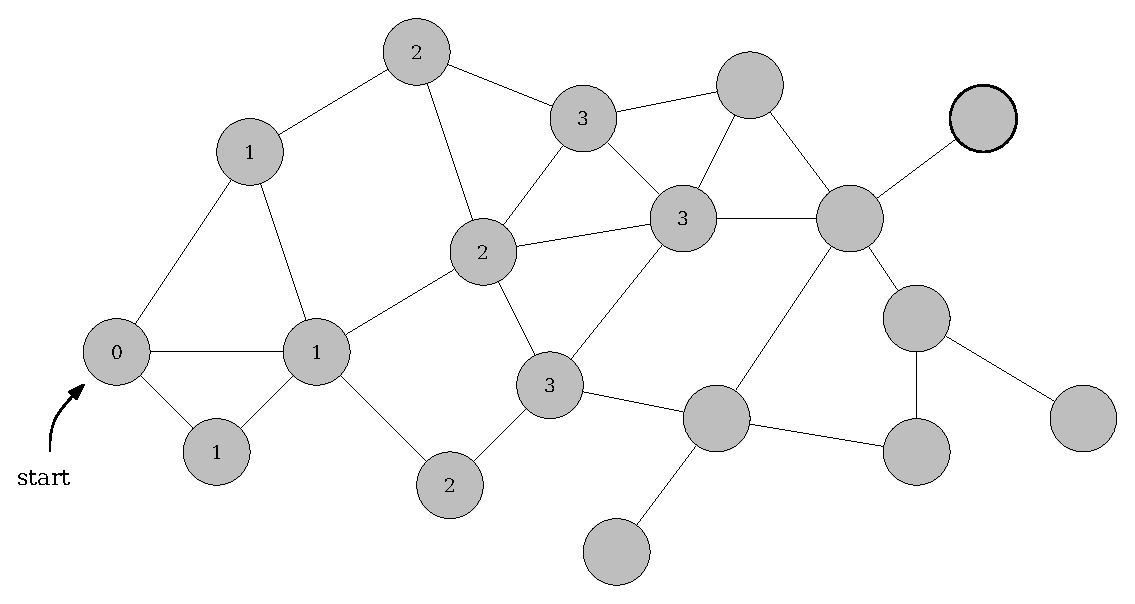
\includegraphics[width=0.6\textwidth]{./algorithms/breadth-first-search/partial-bfs}
	\caption{\small A partially completed breadth-first search on a graph with no particular target node.}
\end{figure}

\subsection{Applications}

\begin{itemize}
	\item Searching graphs with unit edges.
		Graphs with weighted edges should use the Dijkstra or Floyd-Warshall algorithm.
	\item Finding the shortest path between two given nodes.
	\item Testing a given graph for bipartiteness.
	By applying arbitrary, alternating labels to nodes as they are visited, one can determine if a graph is bipartite if a break in the alternation occurs.
\end{itemize}

\subsection{Example Contest Problem: Hopping Stones}

Contemplating wave-based trigonometric functions down by the river forming the southern edge of Farmer John's property may have kept the cows busy for a little while, but studying cowculus with their mathematics mentors is still on their mind.
They must escape the bounds of the fences.
The problem is that not all of them are able to hop the fence, and none would desire to destroy Farmer John's hard work.

There are a number of large rocks in the river that the cows could use to go around the edge of the fencing.
However, many of the cows are queasy about being over the deep waters that it holds and would rather hop around as little as possible.

Reassure the hesitating cows by finding the length of the shortest route possible for them to cross.

\subsubsection{Input}
\begin{itemize}
	\item Line 1: An unsigned integer representing the starting position of the cows.
	\item Line 2: An unsigned integer representing the number of the destination to be hopped to.
	\item Line 3 to EOF: A pair of unsigned integers representing the stones that can be hopped between.
\end{itemize}

\subsubsection{Sample Input}
\acmlisting[label=Hopping Stones Input, caption=Hopping Stones Input]{./algorithms/breadth-first-search/problems/hopping-stones/hopping-stones.in}

\subsubsection{Output}
Text formatted as in the sample output stating the number of hops that must be made to reach the specified destination.

\subsubsection{Sample Output}
\acmlisting[label=Hopping Stones Output, caption=Hopping Stones Output]{./algorithms/breadth-first-search/problems/hopping-stones/hopping-stones.out}

\subsubsection{Example Solution}
\acmlisting[label=Hopping Stones Solution, caption=Hopping Stones Solution]{./algorithms/breadth-first-search/problems/hopping-stones/hopping-stones.cpp}

\subsubsection{Lessons Learned}
\begin{itemize}
	\item If no target node is specified, the algorithm will completely propogate to all reachable nodes.
		This will result in shortest path calculation for all nodes.
	\item Representing the edges as a pair of unsigned integers is much quicker than using a dedicated struct.
\end{itemize}

\subsection{ACM Contest Problem: Word Ladder\cite{acmsoutheastregional2014}}
A \textit{word ladder} is a puzzle in which you transform one word into another by changing one letter at a time.
But, there's a catch: every word that you form in each step must be in the dictionary!
Here's an example of how to transform \textbf{CAT} into \textbf{GAS}:

\vspace{0.15in}

\begin{center}
\textbf{CAT} $\to$ \textbf{CAR} $\to$ \textbf{WAR} $\to$ \textbf{WAS} $\to$ \textbf{GAS}
\end{center}

\vspace{0.15in}

Of course, you want to use the fewest number of transitions possible.
These puzzles can be tough, and often you'll think to yourself:
''Darn it! If only $[$\textit{some word}$]$ was in the dictionary!''

Well, now is your chance!
Given a dictionary, and a starting and ending word, what ONE single word could you add to the dictionary to minimize the number of steps to get from the starting word to the ending word, changing one letter at a time, and making sure that every word at every step is in the dictionary?

\subsubsection{Input}
Each input will consist of a single test case.
Note that your program may be run multiple times on different inputs.
Each test case will start with a line with a single integer $n$ $(2 \le n \le 1000)$ which indicates the number of words in the dictionary.
The dictionary will follow on the next $n$ lines , with one word per line.
All words will consist of between 1 and 8 capital letters only, and all words in a test case wil be the same length.
The first word in the list will be the starting word of the word ladder, and the second word will be the ending word of the word ladder.

\subsubsection{Output}
Output exactly two lines.
The first line holds the one single word that you would add to the dictionary, and the second holds an integer indicating the minimum number of steps to get from the starting word to the ending word, adding your word. Output no spaces.

It is possible that there's more than one word you can add that will make your path as short as possible.
In this case, output the solution word that comes first alphabetically.

It is possible that there's no word you can add that makes the solution possible.
In this case, output $0$ (zero) as the word, and $-1$ as the number of steps.

\section{Depth-first Search}
\index{depth-first search}
\index{search!depth-first}
\index{DFS}

Depth-first search is a method of searching a graph for the possibility reaching a specified node.
As its name suggests, the algorithm will proceed from the starting node to the farthest node of a graph before branching to other nodes.
Because of this, depth-first search is \textbf{not} guaranteed to find the shortest path.
Rather, it will find \textbf{a} path if it exists.
Traversing an entire graph takes $\Theta (m + n)$ for a graph of $m$ vertices and $n$ edges.

\subsection{Applications}
\begin{itemize}
	\item Testing if two graphs are connected by some common node.
	\item Discovering whether a specified state is possible with certain steps.
	\item Finding connected and strongly connected components in $O(m + n)$ time.
\end{itemize}

\subsection{Example Contest Problem: Shaky Stones}
For a while now, the cows have been circumventing the new fence Farmer John built by traversing large rocks that are embedded in the river by the farm.
Some of the stones have become unstable after the cows have used them a number of times.
The ones that are likely to move or sink away have been pointed out by the perceptive cows and given an estimate of the number of times left the stones can be used.

Once again, it's time for the cows to meet their mathematics mentors, and, to do so this time, they need to use the large rocks to get around the fencing.
The cows know which rocks should not be used after a number of times.

Inform the cows of whether they'll all be able to make it, or whether a few need will need to stay behind and be tutored later.

\subsubsection{Input}
\begin{itemize}
	\item Line 1: The number of cows needing to cross.
	\item Line 2: The number of stones that can be used for crossing.
	\item Line 3: The assigned number of the stone the cows start at.
	\item Line 4: The assigned number of the stone the cows finish at.
	\item Line 5: The number of stones, $r$, that have restrictions on them.
	\item Line 6 to $6 + r - 1$: Two integers, the first representing the assigned number of the stone with the restriction on it, and the second representing the number of hops that are deemed safe for it.
	\item Line $6 + r$ to EOF: Two integers representing stones that can be safely hopped between.
\end{itemize}

\subsubsection{Sample Input}
\acmlisting[label=Shaky Stones Input, caption=Shaky Stones Input]{./algorithms/depth-first-search/problems/shaky-stones/shaky-stones.in}

\subsubsection{Output}
\begin{itemize}
	\item Line 1: Print the text 'It is possible.' followed by a newline if the specified number of cows can cross.
		Otherwise, print the text 'It is not possible. Only $x$ can cross' where $x$ is the number of cows that can cross.
\end{itemize}

\subsubsection{Sample Output}
\acmlisting[label=Shaky Stones Output, caption=Shaky Stones Output]{./algorithms/depth-first-search/problems/shaky-stones/shaky-stones.out}

\subsubsection{Example Solution}
\acmlisting[label=Shaky Stones Solution, caption=Shaky Stones Solution]{./algorithms/depth-first-search/problems/shaky-stones/shaky-stones.cpp}

\subsubsection{Lessons Learned}
\begin{itemize}
	\item Depth-first search could also be implemented using a stack in place of where breadth-first search would use a queue.
	\item The algorithm can be written using a while-loop instead of recursion.
\end{itemize}


\chapter{Approaches}
\section{Hash Window Approaches}\index{hashing}\index{hash windows}
Hashing is a mapping of objects to bytes.
These bytes are often stored in Strings or numeric data types.
Normally, hash functions attempt to map each object to a \textit{unique} set of bytes.
Also a \textit{slight} change in the object should cause a \textit{large} change in the output.
When two objects map to the same set of bytes, it is referred to as a hash collision.

\subsection{Approaches}
\begin{itemize}
	\item Identify substrings quickly and cleanly.
	\item Hash collisions to detect certain features of the input.
\end{itemize}

\subsection{Fine Print Returns!}
The cows have prepared another legal document for Farmer John to review.

The Cows are still championing the installation of an Olympic style swimming pool.
However, this time Farmer John only cares about how many times, `pool' appears in the text.

Help Farmer John determine how many times the text `pool' appears in the document.

\subsubsection{Input}
\begin{itemize}
	\item A stream of text terminated by an EOF representing the legal agreement
\end{itemize}

\subsubsection{Sample Input}
\acmlisting[label=Fine Print Sample Input, caption=Fine Print Sample Input]{./approaches/hashing/problems/fine-print/fine-print.in}

\subsubsection{Output}
\begin{itemize}
	\item 1 integer representing the number of references to the word pool in the text.
\end{itemize}

\subsubsection{Sample Output}
\acmlisting[label=Fine Print Sample Output, caption=Fine Print Sample Output]{./approaches/hashing/problems/fine-print/fine-print.out}

\subsubsection{Sample Solution}
\acmlisting[label=Fine Print Sample Solution, caption=Fine Print Sample Solution]{./approaches/hashing/problems/fine-print/fine-print.cpp}

\subsubsection{Lessons Learned}
\begin{itemize}
	\item There is often more than one way to solve a problem,  checkout the KMP string matching algorithm for another way to solve this problem.
\end{itemize}

\section{Dynamic Programming}\index{Dynamic Programming}
Dynamic Programming is a powerful tool that can be applied to several different types of algorithms.\cite{dppractice}
The basic idea is to save the results of smaller problems and use the results to solve larger problems.

\subsection{Applications}
\begin{itemize}
	\item	Improving runtimes of some other algorithms
	\item	Solving the knapsack in $O(nm)$ time
	\item	Solving the integer knapsack in $O(nm)$ time
	\item	Solving the largest increasing subsequence in $O(n \log n)$ time
	\item	Solving the maximum value sub-array problem in $O(n)$
	\item	Solving the maximum value continuous sub-array problem
\end{itemize}

\subsection{Example Contest Problem: A Knapsack Full of Fireworks}\index{Knapsack}
The cows on Farmer John's Farm are planning on putting on a fireworks show for Farmer John's birthday.

They have pooled all of their loose change, and hope to purchase a collection of fireworks that will maximize  Farmer John's amazement during the show so that he will be more likely to build them a new barn.
Each firework's label helpfully includes a "wow factor" rating explicitly for this purpose.
A high "wow factor" is more desirable than a low one.

Please help the cows determine the maximum "wow factor" they can get for their loose change.

\subsubsection{Input Format}
\begin{itemize}
	\item Line 1: One integer, $N$ $(1 \leq N \leq 100)$, the number of fireworks in the catalog.
   \item Line 2: One integer, $C$ $(1 \leq C \leq 10000)$, the total amount of change that the cows have to spend.
	\item Lines 3..$(N+2)$ Two integers $P,W$ representing the price and wow factor for the fireworks.
\end{itemize}

\subsubsection{Sample Input}
\acmlisting[caption=A Knapsack Full of Fireworks Input, label=A Knapsack Full of Fireworks Input]{./approaches/dp/problems/knapsack/knapsack.in}

\subsubsection{Output Format}
\begin{itemize}
	\item Line 1: A single integer representing the maximum wow factor.
\end{itemize}
\subsubsection{Sample Output}
\acmlisting[caption=A Knapsack Full of Fireworks Output, label=A Knapsack Full of Fireworks Output]{./approaches/dp/problems/knapsack/knapsack.out}

\subsubsection{Example Solution}
\acmlisting[caption=A Knapsack Full of Fireworks Solution, label=A Knapsack Full of Fireworks Solution]{./approaches/dp/problems/knapsack/knapsack.cpp}

\subsubsection{Lessons Learned}
The optimal solution is of the form:
$$W(j) = \max \left\{W(j-1), \max \left\{W(j - p_i) + v_i \right\}\right\}$$
Where $W(0) = 0$

\subsection{Example Contest Problem: A Few Fireworks More}\index{Knapsack!Integer}
The cows have reconsidered their original plan of buying just the fireworks with the greatest total "wow factor".
Instead, they want to incorporate "wow factor" \emph{and} diversity, so the cows have decided to purchase a collection of fireworks that optimizes "wow factor" and includes no more than one of each kind of firework in the catalog.

Please help the cows determine the maximum "wow factor" they can get for their loose change, on the condition that they purchase no more than one of each kind of firework in the catalog.

\subsubsection{Input}
\begin{itemize}
	\item Line 1: One integer, $N$, $(1 \leq N \leq 100)$ the number of fireworks in the catalog.
	\item Line 2: One integer, $C$, $(1 \leq C \leq 10000)$ the number of cents that the cows found.
	\item Lines 3..$(N+2)$ Two integers $P,W$ representing the price and wow factor for the fireworks.
\end{itemize}

\subsubsection{Sample Input}
\acmlisting[caption=A Few Fireworks More Input, label=A Few Fireworks More Input]{./approaches/dp/problems/one-zero/one-zero.in}

\subsubsection{Output Format}
\begin{itemize}
	\item Line 1: A single integer representing the maximum wow factor using each firework at most once
\end{itemize}
\subsubsection{Sample Output}
\acmlisting[caption=A Few Fireworks More Output, label=A Few Fireworks More Output]{./approaches/dp/problems/one-zero/one-zero.out}

\subsubsection{Example Solution}
\acmlisting[caption=A Few Fireworks More Solution, label=A Few Fireworks More Solution]{./approaches/dp/problems/one-zero/one-zero.cpp}

\subsubsection{Lesson Learned}
A similar problem to the knapsack, except each item can be used at most once.  The solution here is to expand the state space.  The optimal solution is of the form
$$M(i,j) = \max \left\{ M(i-1, j) , M(i-1, j- s_i) + v_i \right\}$$
Where $M(0,j) = 0$ and $M(i,0) = 0$

\subsection{Example Contest Problem: The Good, the Bad, the Cowy}\index{Largest Increasing Subsequence}
Farmer John's birthday party went off without a hitch, but the cows are worried that Farmer John isn't yet convinced that he should build the cows a new barn. Just in case, they have decided to put it to a vote whether or not they should bake him a cake as well.
Unfortunately, the cows are all experts in the school of bovine politics, and think that a simple majority vote will simply not do because of the dangers of vote rigging.

Instead, the cows have resorted to a rather odd voting system: each cow votes in some arbitrary order with an integer value, and if the length of largest increasing subsequence of all the votes is greater than half the number of cows, then the cows will bake Farmer John a cake.

Help the cows determine the results of their vote.

\subsubsection{Input}
\begin{itemize}
	\item Line 1: Several integers, separated by spaces, representing the votes of the cows.
\end{itemize}

\subsubsection{Sample Input}
\acmlisting[caption={The Good, the Bad, the Cowy Input}, label={The Good, the Bad, the Cowy Input}]{./approaches/dp/problems/cowy/cowy.in}

\subsubsection{Output Format}
\begin{itemize}
	\item Line 1: ``1'' if the cows have decided to bake a cake, and ``0'' otherwise.
\end{itemize}
\subsubsection{Sample Output}
\acmlisting[caption={The Good, the Bad, the Cowy Output}, label={The Good, the Bad, the Cowy Output}]{./approaches/dp/problems/cowy/cowy.out}

\subsubsection{Example Solution}
\acmlisting[caption={The Good, the Bad, the Cowy Solution}, label={The Good, the Bad, the Cowy Solution}]{./approaches/dp/problems/cowy/cowy.cpp}

\subsubsection{Lesson Learned}
\begin{itemize}
	\item This problem can be solved in $O(n \log n)$ time.
	\item Sometimes you have to check the entire array to find the solution.
	\item $while(cin >> val)$ can be used to read in an uncertain number of values.
\end{itemize}


\chapter{Appendix}
\section{C IO Functions}
Occasionally it is far easier to use the C IO functions to meet an output spec. It is also possible to set the precision and width options via numbers after the present,but before the specifier.  The general form of a specifier is: 

\begin{lstlisting}[label=format code format,caption=Format Codes for printf()]
%[flags][width][.precision][length]specifier
\end{lstlisting}

\begin{table}[h]
	\caption{Format Specifier Codes\cite{cplusplus}}
	\begin{tabularx}{\textwidth}{|l|X|l|} \hline
		Format Code &   Output              &   Example     \\ \hline
		d           &   Signed Int          &   314         \\
		u           &   Unsigned Int        &   314         \\
		o           &   Unsigned Octal      &   472         \\
		x           &   Unsigned hex        &   13a         \\
		X           &   UNSIGNED HEX        &   13A         \\
		f           &   floating point      &   3.140000    \\
		e           &   Scientific notation &   3.140000e+00\\
		c           &   character           &   A           \\
		s           &   string              &   ACM         \\
		p           &   pointer address     &   0x40060c    \\
		l           &   Used with other specifiers to indicate a long & 314 \\
		\%\%        &   Prints a literal \% &   \%          \\
		\hline
	\end{tabularx}
\end{table}

\begin{table}[h]
	\caption{Modifier Flags \cite{cplusplus}}
	\begin{tabularx}{\textwidth}{|l|X|l|} \hline
		Format Code &   Output                  &   Example    \\ \hline
		-           &   Left-justify            &   314        \\
		+           &   Force-sign character    &   +314       \\
		\#          &   Show prefix             &   0x13a      \\
			  &   Show decimal point      &   314.       \\
		0           &   Left pad field with 0   &   0314       \\
		\hline
	\end{tabularx}
\end{table}

\subsection{Examples}
\acmlisting[language=c++]{./general/ciofunctions/ciofunctions.cpp}

\section{Some Basic VIMRC Settings}
\acmlisting[language={}, label=vimrc,caption=vimrc]{./general/vimrc/vimrc.example}

\section{Makefile}
\acmlisting[language={}, label=makefile, caption=makefile]{./general/makefile/makefile.example}


\bibliographystyle{plain}
\bibliography{hackpack}

\printindex

\end{document}

